\section{Introduction (WIP)}
\label{sec:introduction}

\begin{itemize}
  \item As a motivation for the work: program verification, \textbf{safety} and why we care about it.
  \item Iris is a new separation logic which allows proving safety for programs using mutable shared state.
        \begin{itemize}
          \item A separation logic allows reasoning about resources that can only be used once.
          \item Iris' concept of ghost state. It's a representation of the program state on a logical level.
          \item persistent resources represent \emph{knowledge} and are freely duplicable.
          \item \emph{shared invariants} represent resources that always exist. It is allowed to take a resource out of an invariant for one atomic step of computation, if the invariant is fixed up in the end.
        \end{itemize}
  \item Many programs nowadays user user-level concurrency to handle a big number of tasks. As an example for \ocf{} there exists the Eio library which provides concurrency primitives using effect handlers.
  \item Effect handlers are a versatile concept which allow a modular treatment of effects, the implementation in form of a handler is separated from the code using the effect, and it's more lightweight than monads. Give a simple example of state.
        \begin{itemize}
          \item The biggest upside is that they are more composable than monads which often require rewriting of parts of the program into monadic style
          \item In theory effect can be tracked by the type system, although \ocf{} does not do that yet.
          \item Explain the concept of \textbf{effect safety} here.
          \item Explain how performing and handling effects is implemented using delimited continuations.
          \item Mention that continuations can only be invoked once? (not really necessary info)
        \end{itemize}
  \item We want to verify some parts of the Eio library but the standard Heaplang language for Iris does not support effect handlers.
        \begin{itemize}
          \item \hazel{} is an Iris language formalizing effect handlers using protocols.
          \item Syntax and semantics of protocols.
          \item Since \ocf{} allows both effect handlers and mutable shared state we had to add a multithreaded semantics to \hazel{}.
        \end{itemize}
  \item Inherent part of a scheduler is liveness, because it is responsible for running all fibers to completion. Unfortunately it is hard to prove liveness properties in Iris, so we just focus on safety and effect safety.
\end{itemize}

\subsection{The Eio Library (WIP)}
\label{sec:intro-eio}

\begin{itemize}
  \item Library for cooperative concurrency in \ocf{}.
  \item Implements switching between tasks using effect handlers.
  \item A fiber is a normal OCaml function which may perform effects that are handled by a scheduler.
  \item Each scheduler is only responsible for a single thread, more can be spawned.
  \item It offers abstractions to operating system resources to fibers, e.g. network, file system, timers etc.
  \item It also offers synchronization and message passing constructs like mutexes \& channels which are specialized to handle fibers, i.e. a mutex does not suspend the system-level thread, but the fiber.
\end{itemize}

\subsection{Focus and Structure of the Thesis}
\label{sec:intro-structure}

Eio aims to be the standard cooperative concurrency library for \ocf{}, so it includes many functions for structured concurrency of fibers (e.g. \ocamlin{Fiber.{first, any, both, all}}, which run two or more fibers and combine their results), support for cancelling fibers, abstractions for operating system resources, a different scheduler implementation per OS, and synchronization constructs like promises and mutexes.
But for this work we restrict ourselves to verifying the safety and effect safety of Eio's core functionalities:
\begin{enumerate}
  \item Running fibers in a "common denominator" scheduler that does not interact with any OS resources,
  \item awaiting the result of other fibers using the \emph{promise} synchronization construct,
  \item and spawning new schedulers to run fibers in another thread.
\end{enumerate}

\begin{figure}[ht]
  \centering
  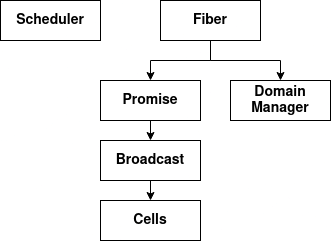
\includegraphics[width=0.75\textwidth]{Eio_Module_Hierarchy.png}
  \caption{Eio Module Hierarchy}
  \label{fig:eio-module-hierarchy}
\end{figure}

Figure~\ref{fig:eio-module-hierarchy} shows the simplified module hierarchy of the concepts we focus on.
A standard arrow stands for a direct source code dependency from one module to another.
The diamond arrow between \ocamlin{Scheduler} and \ocamlin{Fiber} stands for the implicit dependency that code in the fiber module performs effects that are handled by code in the scheduler module.

Fibers can fork off new fibers using the \efork{} effect and suspend execution using the \esuspend{} effect, which are both handled by the scheduler.
The implementation of the fiber and scheduler functions are discussed in section~\ref{sec:sched-impl}.
\emph{Promises} are built on top of the \emph{CQS} data structure, which is a lock-free condition variable that is used by fibers to suspend execution until a promise is fulfilled.
The specification of promises is discussed in section~\ref{sec:sched-spec}.
The CQS specification is already verified using Iris, but Eio uses a custom implementation for which we had to adapt the proof and we discuss this process in section~\ref{sqc:broadcast}.
Fibers in Eio also have access to \emph{thread-local variables} by performing a \egetctx{} effect, which is discussed in section~\ref{sec:thread-local-vars}.
They are thread-local in the sense that they are shared between all fibers of one scheduler.
Finally, we discuss our addition of multi-threading to the \hazel{} operational semantics in order to model running schedulers in different threads.
This turned out to be technically trivial, so we only discuss it in appendix~\ref{sec:apdx-mt} and take a multithreaded semantics and support for Iris \emph{shared invariants} as a given in the reminder of the main text.

\subsection{Contributions}
\label{sec:intro-contributions}

To summarize our contributions, in this thesis we verify the \textbf{safety} and \textbf{effect safety} of a simplified model of Eio which serves as an extended case study on the viability of \hazel{} for verifying programs with effect handlers.
This includes:

\begin{itemize}
  \item The verification of the basic Eio \textbf{fiber abstraction} running on a common denominator scheduler.
  \item An adaptation of the existing verification of CQS to the customized version used by Eio.
  \item Adding multi-threading to \hazel{}'s operational semantics, which shows we can reason about programs that use both \textbf{multi-threading} and \textbf{effect handlers}.
\end{itemize}
